\subsection{Differences of networks analysis} \label{subsec:dc_network_training_methods}

\begin{figure}[t]
\centering

%------------------ Example A: image_030 ------------------
% Left: original (spans the height of two rows)
\begin{minipage}[c]{0.16\linewidth}
  \centering
  
\includegraphics[width=\linewidth]{figures/mnist_split_ic_saliency/image_030_true_3_pred_3/original.png}\\[-2pt]
  {\scriptsize Original}
\end{minipage}\hspace{0.01\linewidth}%
% Right: two rows of five logits
\begin{minipage}[c]{0.81\linewidth}
  \centering
  % Row 1: logits 0..4
  \begin{minipage}[b]{0.19\linewidth}\centering
    
\includegraphics[width=\linewidth]{figures/mnist_split_ic_saliency/image_030_true_3_pred_3/final_saliency_threshold_wrt_0_bright.png}\\[-2pt]{\scriptsize Logit 0}
  \end{minipage}%
  \begin{minipage}[b]{0.19\linewidth}\centering
    
\includegraphics[width=\linewidth]{figures/mnist_split_ic_saliency/image_030_true_3_pred_3/final_saliency_threshold_wrt_1_bright.png}\\[-2pt]{\scriptsize Logit 1}
  \end{minipage}%
  \begin{minipage}[b]{0.19\linewidth}\centering
    
\includegraphics[width=\linewidth]{figures/mnist_split_ic_saliency/image_030_true_3_pred_3/final_saliency_threshold_wrt_2_bright.png}\\[-2pt]{\scriptsize Logit 2}
  \end{minipage}%
  \begin{minipage}[b]{0.19\linewidth}\centering
    
\includegraphics[width=\linewidth]{figures/mnist_split_ic_saliency/image_030_true_3_pred_3/final_saliency_threshold_wrt_3_bright.png}\\[-2pt]{\scriptsize Logit 3}
  \end{minipage}%
  \begin{minipage}[b]{0.19\linewidth}\centering
    
\includegraphics[width=\linewidth]{figures/mnist_split_ic_saliency/image_030_true_3_pred_3/final_saliency_threshold_wrt_4_bright.png}\\[-2pt]{\scriptsize Logit 4}
  \end{minipage}

  \vspace{0.12cm}

  % Row 2: logits 5..9
  \begin{minipage}[b]{0.19\linewidth}\centering
    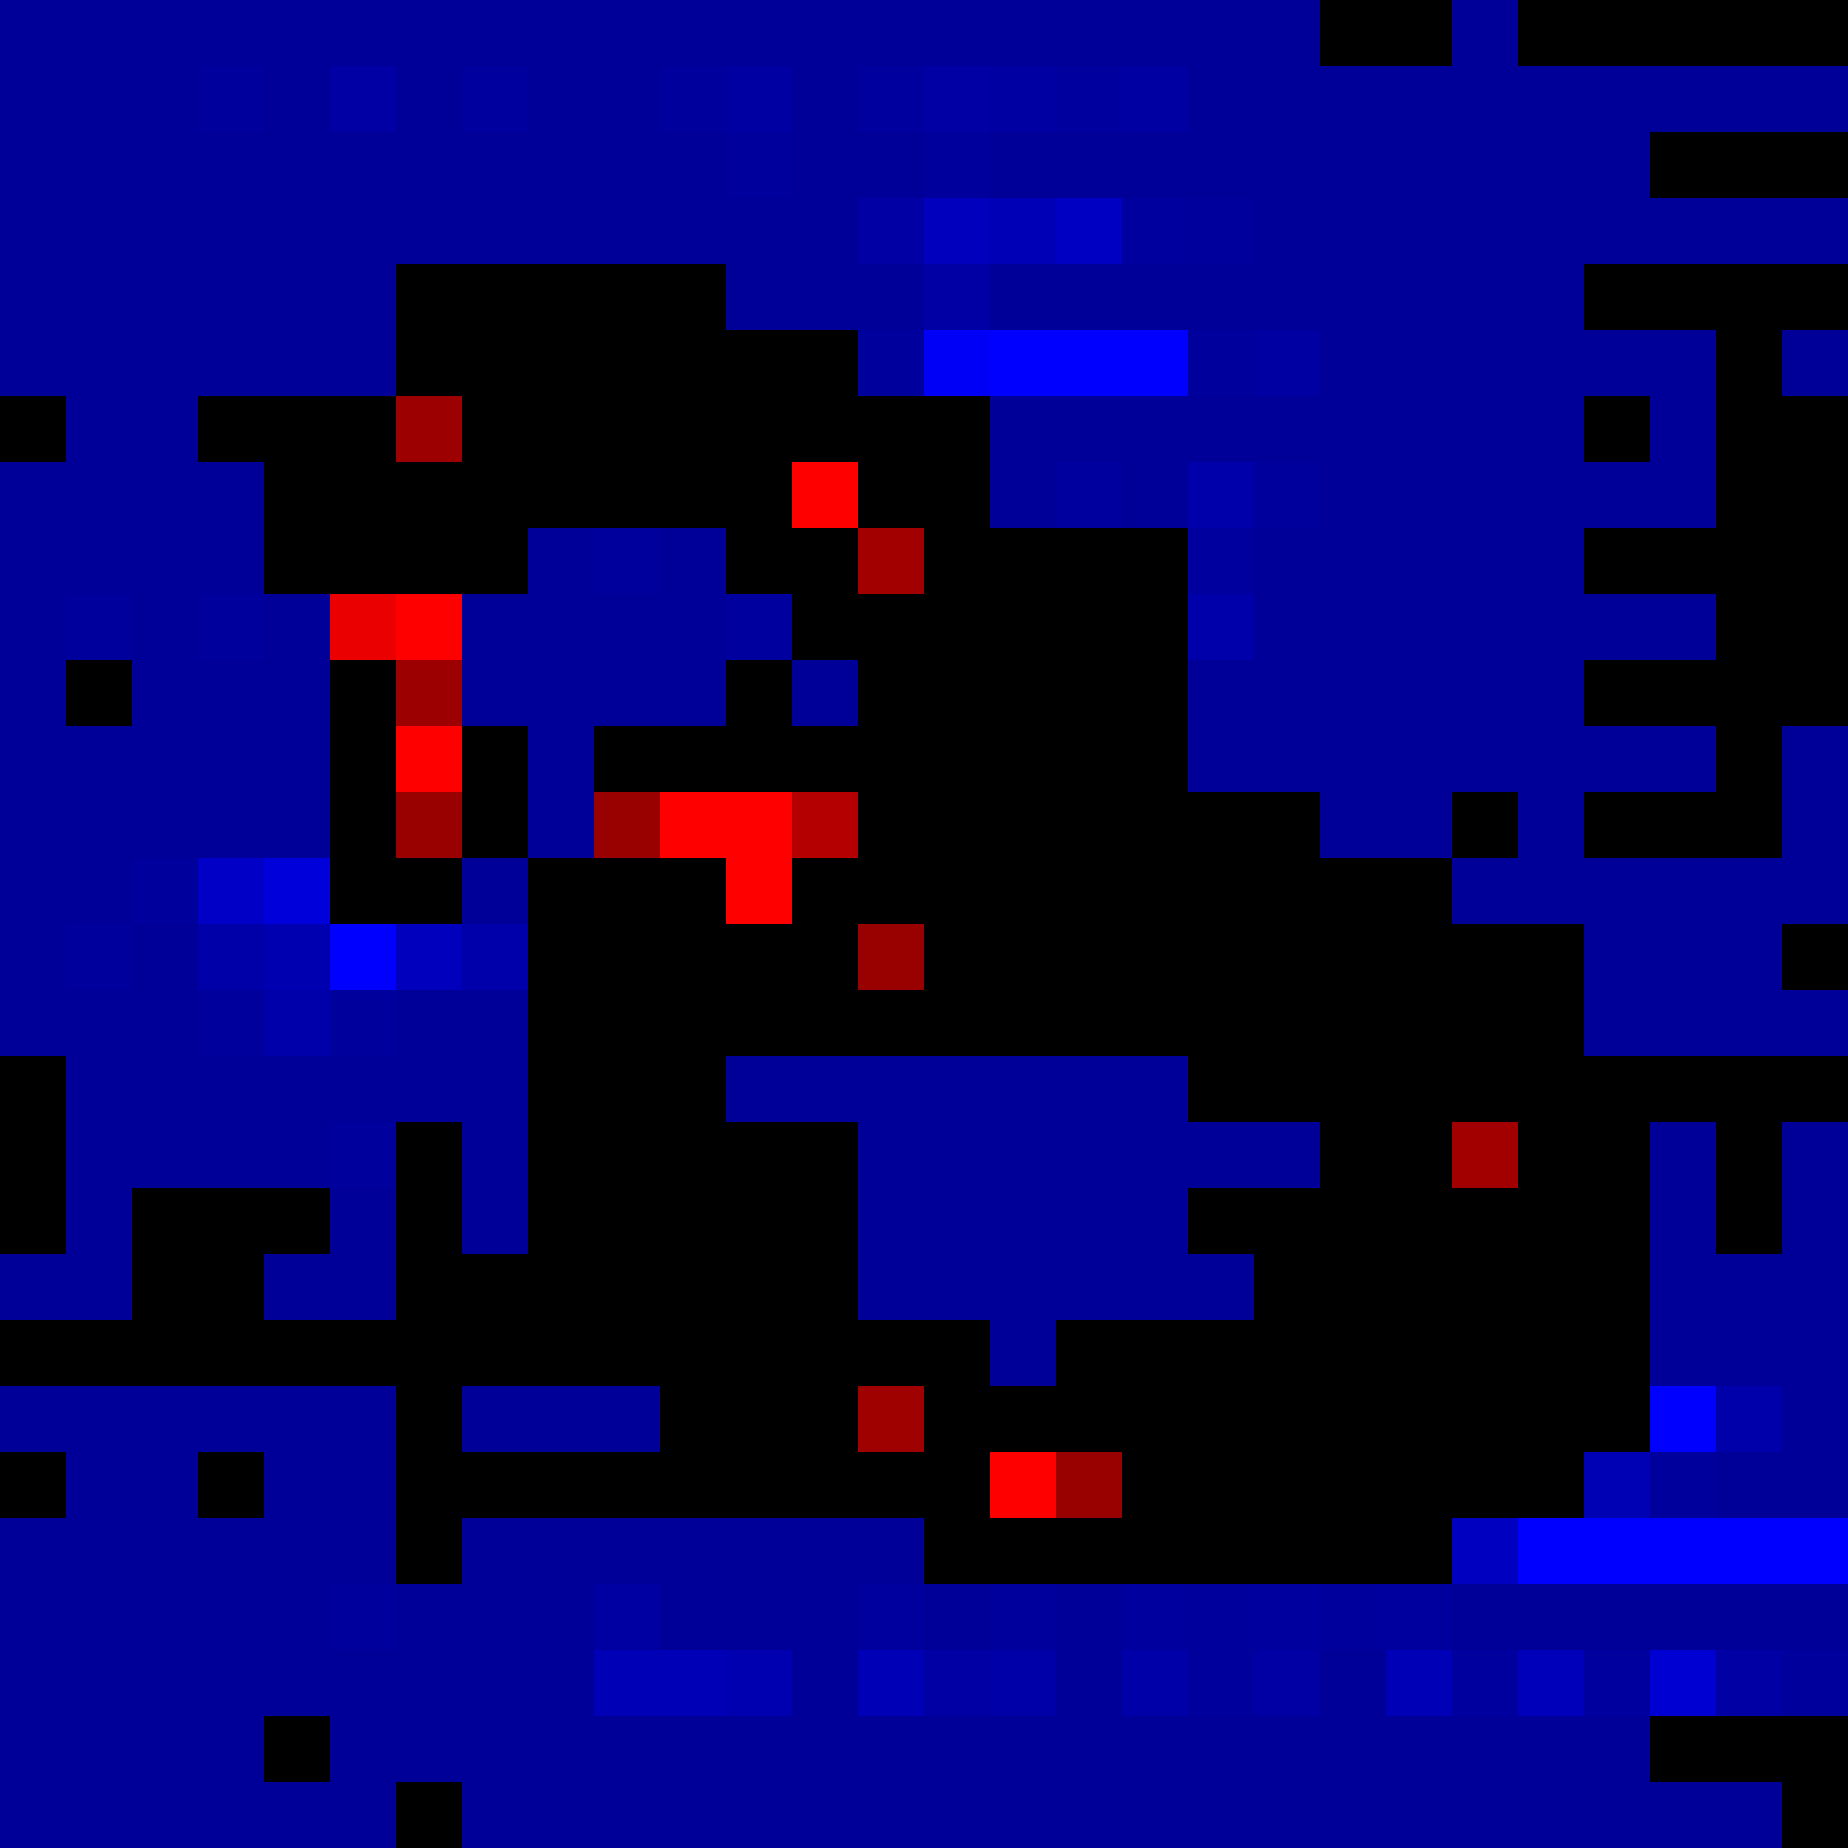
\includegraphics[width=\linewidth]{figures/mnist_split_ic_saliency/image_030_true_3_pred_3/final_saliency_threshold_wrt_5_bright.png}\\[-2pt]{\scriptsize Logit 5}
  \end{minipage}%
  \begin{minipage}[b]{0.19\linewidth}\centering
    
\includegraphics[width=\linewidth]{figures/mnist_split_ic_saliency/image_030_true_3_pred_3/final_saliency_threshold_wrt_6_bright.png}\\[-2pt]{\scriptsize Logit 6}
  \end{minipage}%
  \begin{minipage}[b]{0.19\linewidth}\centering
    
\includegraphics[width=\linewidth]{figures/mnist_split_ic_saliency/image_030_true_3_pred_3/final_saliency_threshold_wrt_7_bright.png}\\[-2pt]{\scriptsize Logit 7}
  \end{minipage}%
  \begin{minipage}[b]{0.19\linewidth}\centering
    
\includegraphics[width=\linewidth]{figures/mnist_split_ic_saliency/image_030_true_3_pred_3/final_saliency_threshold_wrt_8_bright.png}\\[-2pt]{\scriptsize Logit 8}
  \end{minipage}%
  \begin{minipage}[b]{0.19\linewidth}\centering
    
\includegraphics[width=\linewidth]{figures/mnist_split_ic_saliency/image_030_true_3_pred_3/final_saliency_threshold_wrt_9_bright.png}\\[-2pt]{\scriptsize Logit 9}
  \end{minipage}
\end{minipage}

\caption{Combined visualization of the inverted-input DIC stream gradients. The $g$-stream gradient (red) highlights sensitivities on present strokes, while the $h$-stream gradient (blue) highlights sensitivities at candidate missing-stroke locations. These stream-local maps do not by themselves establish the effect of adding pixels on the complete model. On the left: the original digit.}
\label{fig:mnist_split_ic_saliency_main}
\end{figure}


We train two base architectures on MNIST, \texttt{cnn\_maxout} and \texttt{mlp\_maxout}, and their difference-of-two variants.
The \textbf{DIC-model} (directly trained as the difference of two input-convex neural networks) denotes $g-h$ with both streams input-convex, while the \textbf{DM-model} (directly trained as the difference of two monotone networks) denotes $g-h$ with both streams monotone.
For each base model we also evaluate the \emph{inverted-input} variant (DIC\-IN / DM\-IN), where the $h$-stream processes $1-x$ so it can better focus on missing features.
Implementation-wise, positivity is enforced by parameterizing all constrained weights and affine terms via a nonnegativity transform, and batch norm parameters are constrained analogously.

On \texttt{mlp\_maxout}, DIC-models and DM-models slightly improve test accuracy over their single-stream counterparts.
The complete evaluation and more training details can be found in \cref{app:explaining_io_convex_nns}.
\cref{fig:mnist_split_ic_saliency_main} demonstrates the seperation of the two DIC models to focus on present and missing stroke features respectively.